\documentclass[LaTeX2e,10pt,aspectratio=169]{beamer}

\usepackage{xcolor}
\usepackage{graphicx}
\usepackage{psfrag}
\usepackage{epstopdf}
\usepackage{hyperref}
\usepackage{bookmark}
\usepackage{svg}
\usepackage{fontspec}

\setmainfont{Lucida Sans}
\setsansfont{Lucida Sans}
\setmonofont{Lucida Sans}
\newfontfamily{\georgia}{Georgia}

%%%% NEUTRAL COLOUR PALETTE %%%%%
\definecolor{sotonPlainBlack}{HTML}{231F20} % soton plain black
\definecolor{sotonRichBlack}{HTML}{00131D}  % soton rich black (litho print only)
\definecolor{sotonNeutral1}{HTML}{495961}   % neutral 1
\definecolor{sotonNeutral2}{HTML}{758D9A}   % neutral 2
\definecolor{sotonNeutral3}{HTML}{9EB1BD}   % neutral 3
\definecolor{sotonNeutral4}{HTML}{E1E8EC}   % neutral 4

%%%% MARINE COLOUR PALETTE %%%%%
% Note: per the latest brand update, the old "Prussian" became Marine 1,
% and the old Marine 1 became University Blue.
\definecolor{sotonUniversityBlue}{HTML}{005C84} % university blue
\definecolor{sotonMarine1}{HTML}{002F4C}        % marine 1 (formerly Prussian)
\definecolor{sotonMarine2}{HTML}{0C838C}        % marine 2
\definecolor{sotonMarine3}{HTML}{74C9E5}        % marine 3
\definecolor{sotonMarine4}{HTML}{83DBD2}        % marine 4
\definecolor{sotonMarine5}{HTML}{4BB694}        % marine 5
\definecolor{sotonMarine6}{HTML}{C0D100}        % marine 6

%%%% HORIZON COLOUR PALETTE %%%%%
\definecolor{sotonHorizon1}{HTML}{FCBC00} % horizon 1 - yellow
\definecolor{sotonHorizon2}{HTML}{EF7D00} % horizon 2 - orange
\definecolor{sotonHorizon3}{HTML}{E63037} % horizon 3 - red
\definecolor{sotonHorizon4}{HTML}{D5007F} % horizon 4 - magenta/pink
\definecolor{sotonHorizon5}{HTML}{8D3970} % horizon 5 - purple

%%%% TEMPLATE-SPECIFIC COLOURS %%%%%
\definecolor{sotonContentBg}{HTML}{F9FBFF}   % off-white content slide background
\definecolor{sotonTitleText}{HTML}{2E444E}    % dark slate used for titles/body on light slides

% ----------------------------- COLOUR ASSIGNMENT -----------------------------------------------
% Content slides: off-white background, dark slate titles/body, neutral1 bullets
\setbeamercolor{background canvas}{bg=sotonContentBg}
\setbeamercolor{normal text}{fg=sotonNeutral1}
\setbeamercolor{title page}{fg=white}

\setbeamercolor{block title}{fg=sotonUniversityBlue}
\setbeamercolor{frametitle}{fg=sotonTitleText}
\setbeamercolor{framesubtitle}{fg=sotonNeutral1}
\setbeamercolor{alerted text}{fg=sotonHorizon3}
\setbeamercolor{titlelike}{fg=sotonTitleText}
\setbeamercolor{author}{fg=sotonNeutral1}
\setbeamercolor{date}{fg=sotonNeutral1}
\setbeamercolor{item}{fg=sotonNeutral1}
\setbeamercolor{caption name}{fg=sotonNeutral1}
\setbeamercolor{footline text}{fg=sotonNeutral1}
\setbeamercolor{page number in head/foot}{fg=sotonNeutral1}

% Bullet characters to match the brand template (• level 1, -- level 2)
\setbeamertemplate{itemize item}{\textbullet}
\setbeamertemplate{itemize subitem}{--}
\setbeamercolor{itemize item}{fg=sotonNeutral1}
\setbeamercolor{itemize subitem}{fg=sotonNeutral1}

% Edit the margins:
\setbeamersize{text margin left=1.2cm, text margin right=1.2cm}

% Fonts:
\setbeamerfont{title}{size={\fontsize{16pt}{18pt}}}
\setbeamerfont{subtitle}{size={\fontsize{10pt}{12pt}}}
\setbeamerfont{author}{size={\fontsize{10pt}{12pt}}}
\setbeamerfont{institute}{size={\fontsize{10pt}{12pt}}}
\setbeamerfont{date}{size={\fontsize{10pt}{12pt}}}
\setbeamerfont{frametitle}{size={\fontsize{16pt}{18pt}}}
\setbeamerfont{framesubtitle}{size={\fontsize{10pt}{12pt}}}
\setbeamerfont{normal text}{size={\fontsize{10pt}{12pt}}}
\setbeamerfont{itemize item}{size={\fontsize{10pt}{21pt}}}
\setbeamerfont{itemize subitem}{size={\fontsize{9pt}{21pt}}}

\newcommand{\putlogoWhite}{\includesvg[width=3.5cm]{Logos/USH0149_LOGO-2021_RGB_White_Punched-AW.svg}}
\newcommand{\putlogoBlue}{\includesvg[width=3.5cm]{Logos/USH0149_LOGO-2021_RGB_Marine-Blue_Punched-AW.svg}}
\newcommand{\putlogoNeutral}{\includesvg[width=3.5cm]{Logos/USH0149_LOGO-2021_RGB_Neutral_Punched-AW.svg}}
\newcommand{\putlogoBlack}{\includesvg[width=3.5cm]{Logos/USH0149_LOGO-2021_RGB_Black_Punched-AW.svg}}

\newcommand{\footline}{\color{sotonNeutral3}\rule{\textwidth}{1pt}}

% ----------------------------- TITLE PAGE -----------------------------------------------------
\setbeamertemplate{title page}{
	\vskip50pt
	\hspace{18pt}
	\begin{minipage}{0.78\textwidth}
		\raggedright
		{\usebeamerfont{title}\usebeamercolor[fg]{title page}\inserttitle}\\[4pt]
		{\usebeamerfont{subtitle}\usebeamercolor[fg]{title page}\insertsubtitle}
		\vskip18pt
		{\usebeamerfont{author}\usebeamercolor[fg]{title page}\insertauthor}
		\vskip12pt
		{\usebeamerfont{date}\usebeamercolor[fg]{title page}\insertdate}
	\end{minipage}
}
% ----------------------------- END ----------------------------------------------------------------

\title{Turbine Blade Design in the Face of Uncertainty}
\author[WJ]{William Jacques$^1$, 2nd author$^2$\\~\\ \footnotesize $^1$University of Southampton, UK\\$^2$University of Colorado, USA}
\institute[FEE]{Faculty of Engineering and the Environment\\University of Southampton}
% ----------------------------- END ------------------------------------------------------------
% ---------- FURTHER DEFINITIONS --------------
\setlength{\unitlength}{1cm}
\graphicspath{{./Graphics/}}
% --------------- END -------------------------

\begin{document}

% Title slide
{
\setbeamertemplate{background canvas}{\color{sotonUniversityBlue}\rule{\paperwidth}{\paperheight}}
\setbeamertemplate{headline}{
	\vspace{9pt}\hspace{2pt}\hfill\putlogoWhite\hspace{5mm} % logo top-right on title slide
}
\setbeamertemplate{footline}{}
\frame{\titlepage}
\addtocounter{framenumber}{-1} % Do not count the title frame!
}

% Content slides
\setbeamertemplate{headline}{
	\vskip30pt
	\vskip-21pt\hspace{1pt}\hfill\putlogoBlue\hspace{5mm} % blue logo on the right
}

\setbeamertemplate{footline}{
	\vskip-10pt\footline\\ % horizontal line
	\vskip2pt
	\makebox[123mm]{\hspace{7.5mm}
	\insertshorttitle
	\hfill \insertframenumber/\inserttotalframenumber}
	\vskip4pt
}

\setbeamertemplate{frametitle}{
	\usebeamerfont{frametitle}\usebeamercolor[fg]{frametitle}\insertframetitle\\
	\ifx\insertframesubtitle\@empty\else
		{\usebeamerfont{framesubtitle}\usebeamercolor[fg]{framesubtitle}\insertframesubtitle}
	\fi
}

\begin{frame}
	\frametitle{TABLE OF CONTENTS}
	\tableofcontents
\end{frame}

\section{Introduction}

\begin{frame}{GUIDANCE}
\framesubtitle{Subtitles should be sentence case, 20pt}
\begin{itemize}
	\item Body copy is size 20pt with normal letter spacing.
	\item Bullet points have a single line spacing with a 12pt space after
	\begin{itemize}
		\item Secondary bullet points are 18pt
	\end{itemize}
	\item You can also use the {\georgia Georgia} font for emphasis on quotations.
\end{itemize}
\end{frame}

\begin{frame}{INTRODUCTION}
	\vskip7pt
\begin{figure}[h!]
	\centering
	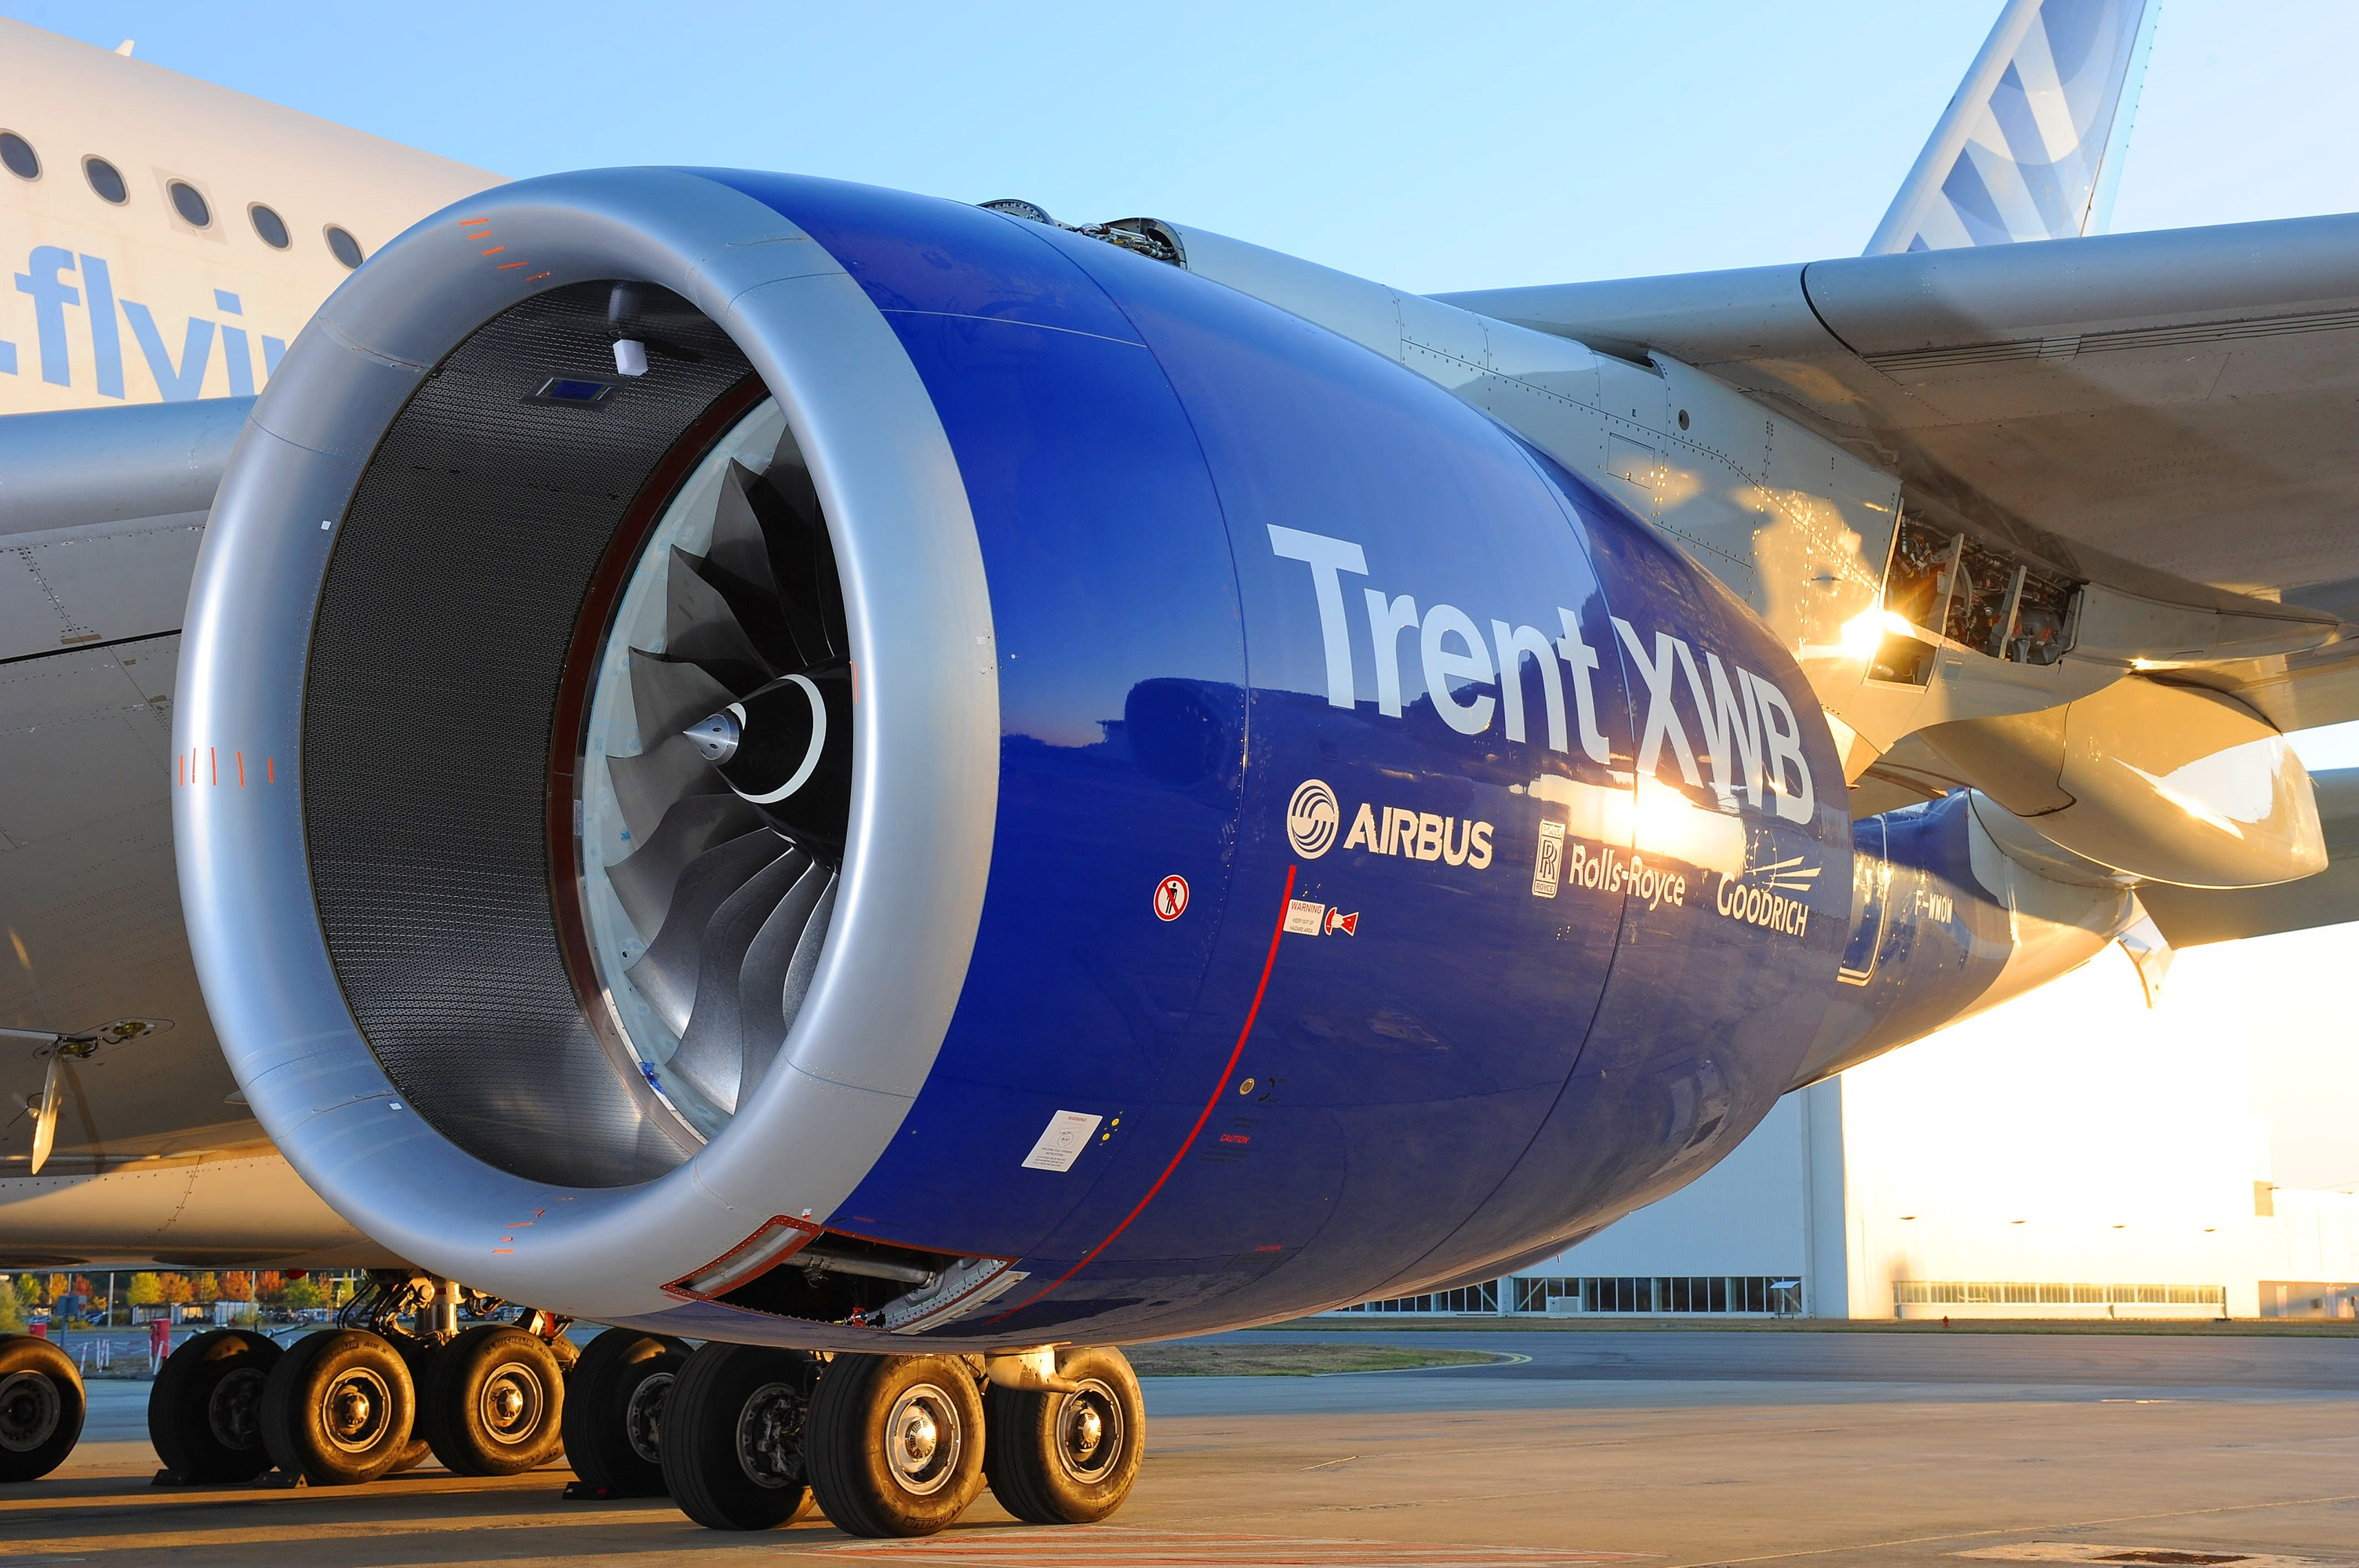
\includegraphics[height=0.4\textwidth]{Graphics/A350_XWB.jpg}
	\caption{Trent XWB turbofan}
	\label{fig:xwb}
\end{figure}
\end{frame}

\begin{frame}{INTRODUCTION}
	\vskip7pt
	\begin{figure}[h!]
		\centering
		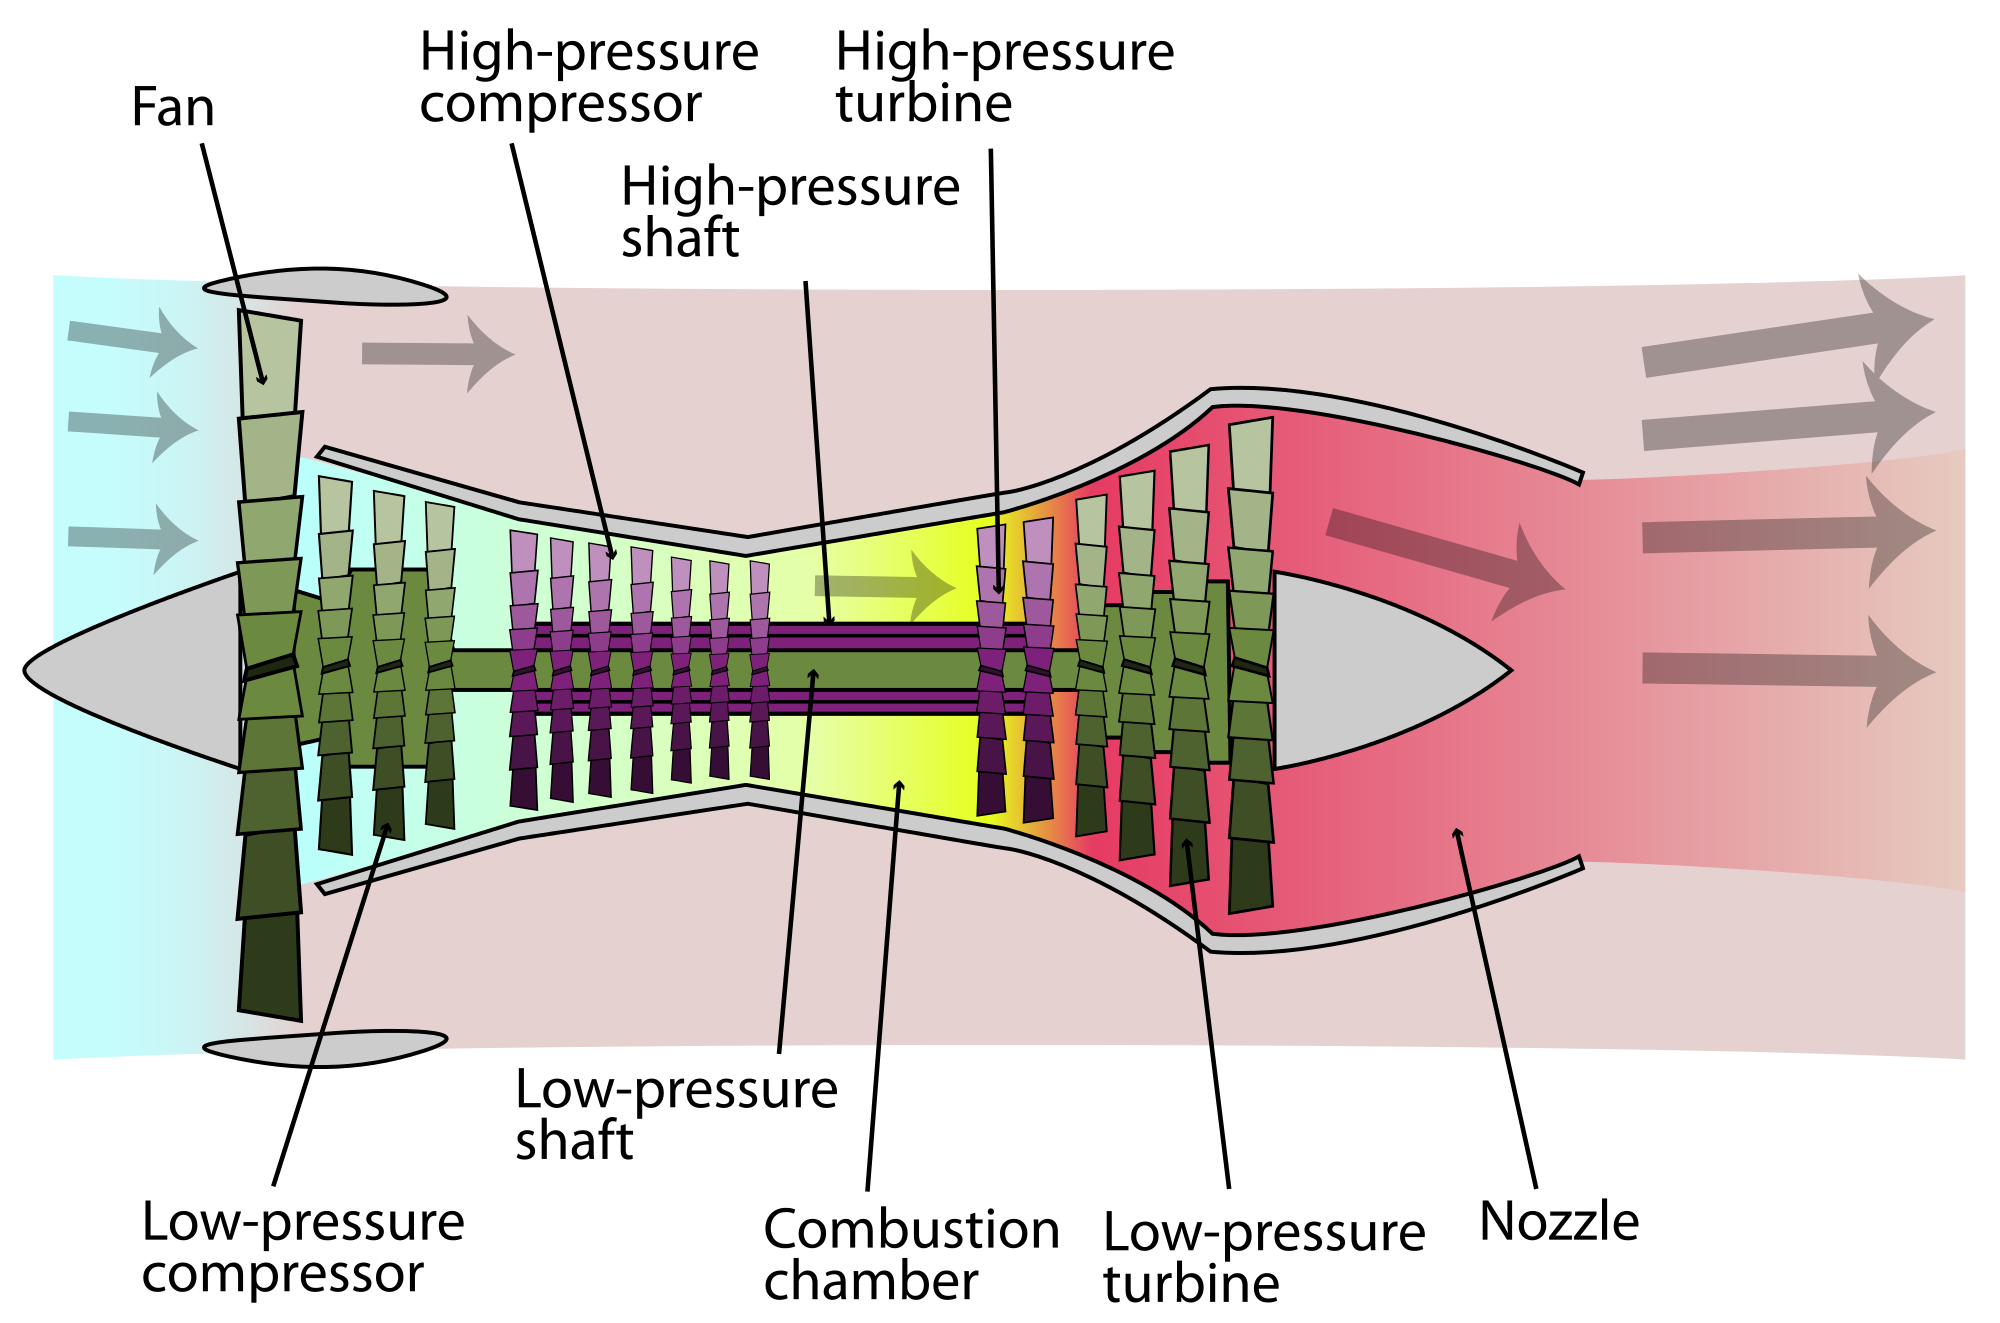
\includegraphics[height=0.4\textwidth]{Graphics/2000px-Turbofan_operation.png}
		\caption{Major components of turbofans}
		\label{fig:turbofan}
	\end{figure}
\end{frame}

\section{Main content}

\begin{frame}{TURBINE BLADES}{This is a subtitle example}
	\begin{enumerate} [<+->]
		\item item 1
		\item item 2
	\end{enumerate}
\end{frame}

\section{Conclusions}

\begin{frame}{CONCLUSIONS}
	Some conclusions
\end{frame}

{
\setbeamertemplate{background canvas}{\color{sotonUniversityBlue}\rule{\paperwidth}{\paperheight}}
\setbeamertemplate{headline}{
	\vspace{4pt}\hspace{2pt}\hfill\putlogoWhite\hspace{3.5mm}
}
\setbeamertemplate{footline}{}
\begin{frame}
	\vskip30pt
	\hspace{18pt}
	{\Large\bfseries\color{white}YOUR QUESTIONS}
\end{frame}
}

\end{document}